\documentclass{beamer}
\usepackage{beamerthemeshadow}
\usepackage{graphicx}
\usepackage{color}
\usepackage[utf8]{inputenc}
\usepackage{hyperref}
\usepackage{tikz}
\usepackage[flushleft]{threeparttable}
\definecolor{beamer@darkred}{rgb}{0.85,0.1,0.1}
\setbeamercolor{structure}{fg=beamer@darkred}

\def\d{{\fontencoding{T1}\selectfont\dj}}
\def\D{{\fontencoding{T1}\selectfont\DJ}}


\title{Medijska pismenost}
\author{Ljiljana Mihajlović, Danica Šimšić,\\ Ana Stevanović, Tijana Zečević}
\institute{Matematički fakultet\\Univerzitet u Beogradu}
\date{
	\footnotesize{Beograd, 2022.}	
}

\begin{document}
\begin{frame}
	\thispagestyle{empty}
	\titlepage
\end{frame}

\addtocounter{framenumber}{-1}

\begin{frame}
	\begin{itemize}
		\item Zasnovano na:\\
		Grupa autora (po azbučnom redu): Vlajković Bojić Violeta, Miladinović Nenad, Milijić Subić Dejana, Milošević Ivana. Priručnik za nastavnike \emph{ Naši učenici u svetu kritičkog mišljenja i medijske pismenosti}.
		(\url{https://zuov.gov.rs/prirucnik-za-nastavnike-nasi-ucenici-u-svetu-kritickog-misljenja-i-medijske-pismenosti/})

  
            Nedim Sejdinović i Tatjana Ljubić, \emph{Osnove medijske pismenosti– priručnik za učenike}, 2014.
            (\url{http://www.medijskapismenost.net/dokument/Osnove-medijske-pismenosti---prirucnik-za-ucenike/})\\
  
	\end{itemize}
\end{frame}

\begin{frame}
	\frametitle{Pregled} % Table of contents slide, comment this block out to remove it
	\tableofcontents[hidesubsections] 
\end{frame}

\section{Tradicionalni i društveni mediji}

\begin{frame}[fragile]\frametitle{Kako ljudi pamte?}
	\begin{itemize}	
		\item 10\% onoga što pročitaju
		\item 20\% onoga što čuju
		\item 30\% onoga što vide
		\item 50\% onoga što čuju i vide
		\item 70\% onoga što kažu i napišu
		\item 90\% onoga što rade
	\end{itemize}
\end{frame}

\section{Spinovanje i manipulacija}

\begin{frame}[fragile]\frametitle{Kako ljudi uče?}
	\begin{itemize}	
		\item Verbalnim putem (čitanjem i slušanjem)
		\item Vizuelnim putem (gledanjem)
		\item Aktivnim učešćem (gledanjem, slušanjem i činjenjem)
	\end{itemize}
\end{frame}


\section{Dezinformacije}
\begin{frame}[fragile]\frametitle{Dezinformacije: vidovi i načini prepoznavanja}
	\begin{itemize}	
		\item podmetnuti sadržaj
		\item obmanjujući sadržaj
		\item fabrikovani sadržaj
  		\item manipulisani sadržaj
	\end{itemize}
 
\begin{tikzpicture}[remember picture, overlay]
\node[above=0.7cm, left=1cm] at (current page.east) 
{
    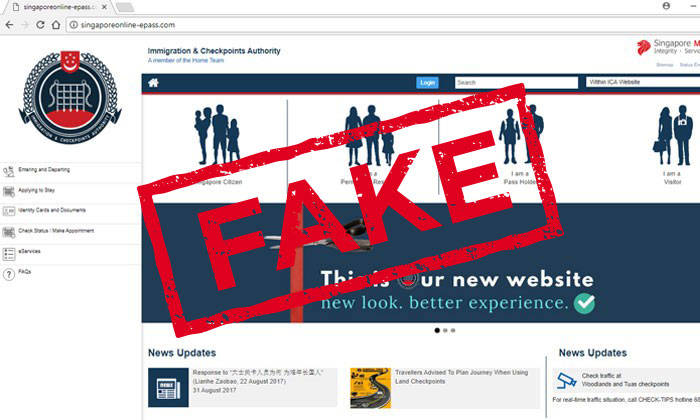
\includegraphics[width=0.5\textwidth]{fakewebsite.jpg}
};
\end{tikzpicture}

\begin{tikzpicture}[remember picture, overlay]
\node[below = 2.65cm, left=1cm] at (current page.0) 
{
    
\includegraphics[width=0.5\textwidth]{takecarebeforeyoushare.jpg}
};
\end{tikzpicture}

\end{frame}

\section{Medijska pismenost u doba informacija}

\begin{frame}[fragile]\frametitle{Kako ljudi uče?}
	\begin{itemize}	
		\item Verbalnim putem (čitanjem i slušanjem)
		\item Vizuelnim putem (gledanjem)
		\item Aktivnim učešćem (gledanjem, slušanjem i činjenjem)
	\end{itemize}
\end{frame}


\section{Zakljucak}

\begin{frame}[fragile]\frametitle{Kako ljudi uče?}
	\begin{itemize}	
		\item https://www.overleaf.com/project/6373cb36fddbf10b53a4c45b
		\begin{itemize}
			\item samo 8\% poruke se prenese samim rečima (verbalna komunikacija)
			\item 37\% se prenesi bojom glasa, tonalitetom, pauzama u govoru (paralingvističkim znakovima)
			\item 55\% poruke se prenosi govorom tela: pratećim pokretima, izrazom lica i
			očiju, stavom tela i drugo (neverbalna komunikacija)
		\end{itemize}
		\item Verbalnim putem se najčešće prenose činjenice i
		sirove informacije, dok se neverbalnim putem prenose stavovi i
		emocionalni odnos prema činjenicama koje izlažemo.
	\end{itemize}
\end{frame}

\end{document}